\documentclass[a4paper]{article}

%% Language and font encodings
\usepackage[english]{babel}
\usepackage[utf8x]{inputenc}
\usepackage[T1]{fontenc}

%% Sets page size and margins
\usepackage[a4paper,top=3cm,bottom=2cm,left=3cm,right=3cm,marginparwidth=1.75cm]{geometry}

%% Useful packages
\usepackage{amsmath}
\usepackage{graphicx}
\usepackage[colorinlistoftodos]{todonotes}
\usepackage[colorlinks=true, allcolors=blue]{hyperref}

\title{Inference on the Evolutionary History of Embryo-Cerebral Related Genes in Metazoan: using a novel Bionformatic Approach.}
\author{Ramirez R. Antonio, Aviña P. Katia, Gómez R. Ricardo, Villegas J. Santiago, Álvarez C. Sebastián, TA: Valdivia M. Dulce}


\begin{document}
\maketitle

\begin{abstract}
Embryo development relies on the complex interplay of the basic cellular processes including proliferation, differentiation, and apoptosis.Regulation of these events is basic for the establishment of structures and organ development.The aim of our project was analyzing the evolutionary history of a set of genes differentially expressed in prosencephalon which is the embryonic structure from which the cerebrum develops prenatally. A novel bioinformatics approach was proposed in order to infer phylogeny trees of orthologous genes among different metazoan species. Our method consisted in a \texttt{ProteinOrtho} analysis followed by a modular decomposition and a reconciliation using \texttt{El Chicken} tool.This approach allowed us to detect biological events as speciation and duplication as well as discard not biological significantly results. Our results shown that this method probe to be useful for the inferencne of the evolutionary history of embryo-cerebral related genes in Metazoan. 


\end{abstract}

\section*{Introduction}
Embryo development relies on the complex interplay of the basic cellular processes including proliferation, differentiation, and apoptosis. Regulation of these events is basic for the establishment of structures and organ development.

Most studies of evolutionary developmental biology has traditionally focus in conservation of developmental processes, mainly related with gene expression patterns (1-2).Differences at the level of genes and gene interactions among metazoan groups have also been studied (3).

Earlier work identified gross developmental similarities and differences between metazoan groups that led to their classification into three types of development (4-6). However, studies so far have not integrated the available genome information with the appropriate bioinformatics tools to infer evolutionary history of brain developmental genes during early stages.

The aim of our project was to analyzed the evolutionary history of a set of genes previously identified as differentially expressed in procenphalon which is the embryonic structure from which the cerebrum develops prenatally in mammals. Our method consisted in a \texttt{ProteinOrtho} analysis (7) followed by a modular decomposition and a reconciliation using \texttt{El Chicken} tool.This novel bioinformatics approach allowed us to understand the similarities and differences in the early process of brain development among metazoa.

This project introduces a \texttt{bioinformatics approach} that infers the information about biological events as duplication and speciation and also allowed us to identify the biological relevance of those genes. We propose new hypotheses about the relationship between embryo brain development orthologous genes in the classification of developmental types. Particular attention is given to the distinction between orthologous genes coming from speciation and duplication events. 

This work suggests that this type of evolutionary events have important implications for our understanding of cerebrum developmental dynamics and how brain development evolutionary history occurred in metazoa. 



\section*{Objectives}
\begin{itemize}
	\item  Infer the evolutionary history of genes associated with the development of the brain in the embryonic stage of metazoan through an orthologous gene functional analysis.
\end{itemize}

\subsection*{Particular Objectives}
\begin{itemize}
	\item Create an orthologous-genes graph from 5 different metazoan genomes using  \texttt{ProteinOrtho} tools.
    \item Determine orthologous genes for a differentially expressed genes (DEG's) during embryonic brain development stage in mouse for further in silico analysis.
    \item Determine gene evolutionary events 	(speciation,duplication)using connected components Networkx analysis and modular decomposition algorithm using an python approach.
    \item Determine a gene ontology (GO) comparative analysis from the phylogenetic tree obtained using our propoused bioinformatic approach.
\end{itemize}

\section*{Methodology}
First, coding sequences from five metazoan genomes ({\it Homo sapiens}, {\it Mus musculus}, {\it Gallus gallus}, {\it Danio rerio} and  {\it Drosophila melanogaster}) were downloaded from Ensembl database
[ensemble.org](http://www.ensembl.org/info/data/ftp/index.html). Those sequences were submitted to \texttt{ProteinOrtho} tool that allowed to infer gene ortologous relationships.

Connected component analysis was performed using \texttt{Networkx} package from \texttt{python} environment results were refined to those related with a set of 1351 genes previously identified as differentially expressed in prosencephalon tissue from {\it Mus musculus}, during 10.5 day of embryo-developmental stage. For modular decomposition a novel programm called \texttt{El Chicken} was used. From the results obtained a scrutiny was performed, criteria for selection was series ({speciation}) and parallels {duplication}. Data shown as prime nudes in the graph was discarded for further analysis. Finally phylogenetics trees comparative analysis was performed to infer the evolutionary history of embryo related genes in metazoan (Fig. 1).


%\section*{Methodology: Bioinformatics Approach}
		\begin{figure}[h]
			\centering
            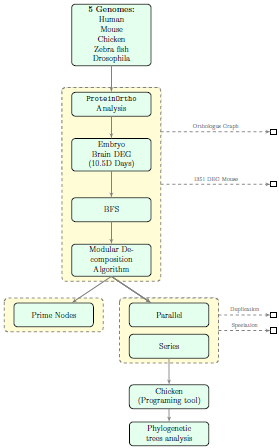
\includegraphics[height = 0.40\textheight]{este.png}
            \caption{Bioinfortmatic Approach: Flow Diagram}
            
		\end{figure}

\section*{Results and Discussion}



\begin{figure}[h]
			\centering
            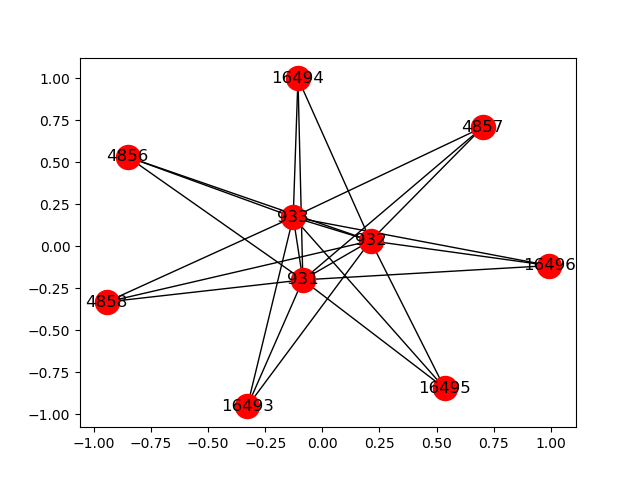
\includegraphics[height = 0.40\textheight]{Figure_1.png}
            \caption{Conected component example}\label{cc}
		\end{figure}

\begin{figure}[h]
			\centering
            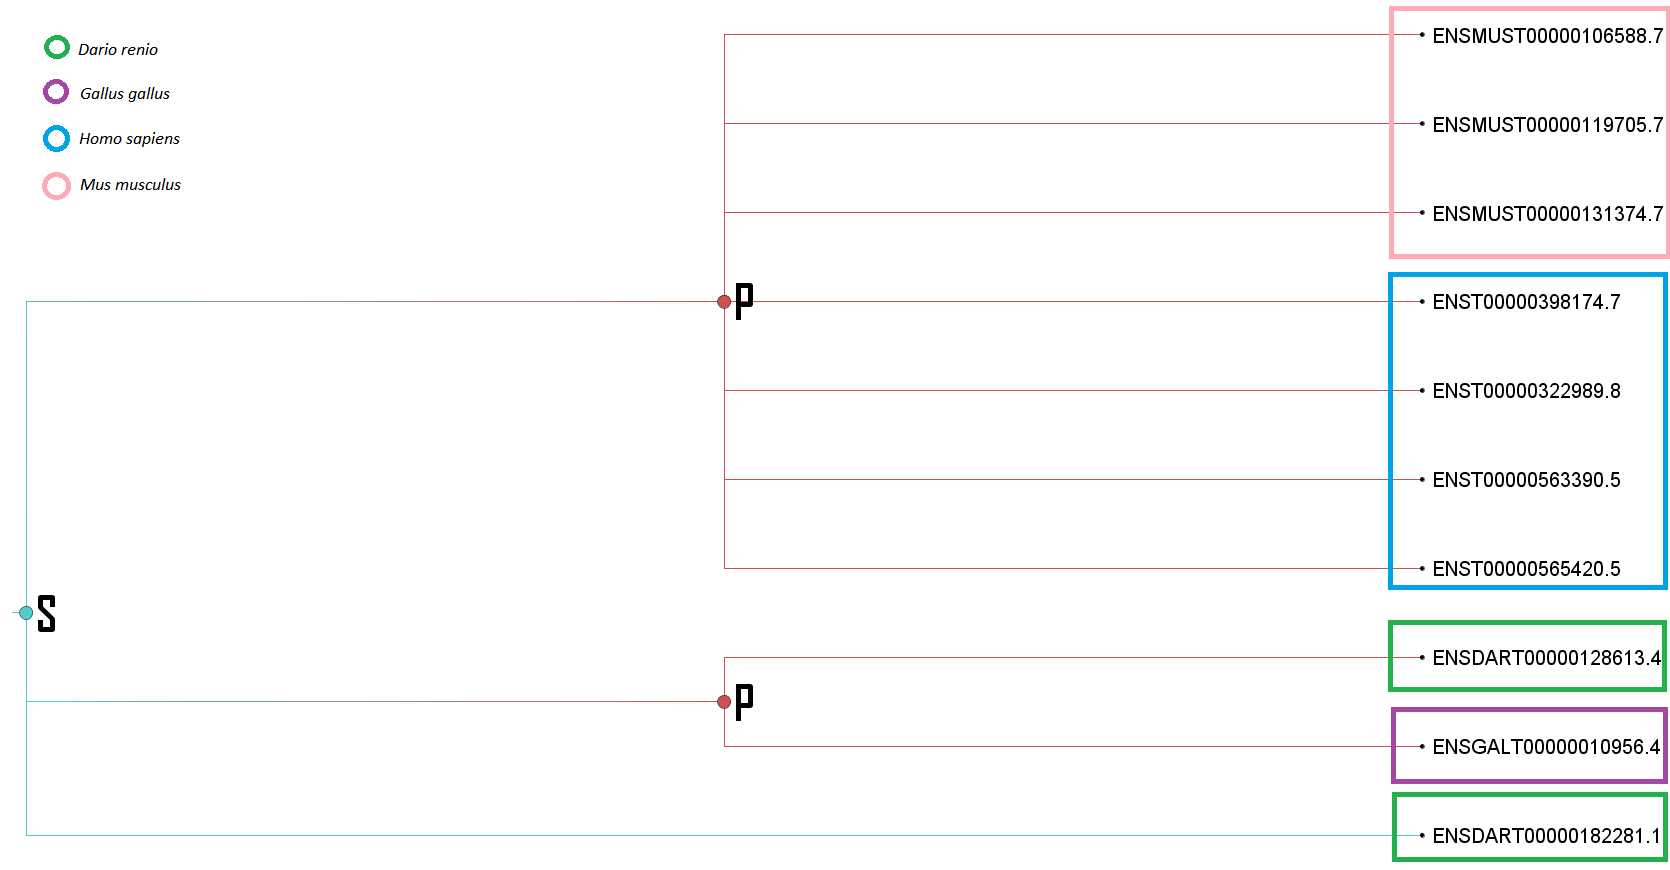
\includegraphics[height = 0.20\textheight]{Arbolbuenoahorasi.png}
            \caption{Phiilogenetic tree}\label{Philogenetic tree}
            
		\end{figure}

Evidence has shown that at this particular stage brain has developed from the anterior end of the nerval tube into three primary vesicles 1)Telencephalic, 2)Mesencephalic and 3)Rhombencephalic. Prosencephalon has been identified as the embryonic structure from which the cerebrum develops prenatally into Telencephalon. Telencephalon has been related with multiple biological functions such as body temperature, reproductive functions, and display of emotions.
 
Our results could help us to distinguished types of development among metazoa, and to proposed hypothesis regarding the connection between developmental type and early brain morphological variation within and between species, and vertebrate evolution.
 
Studies of brain formation and morphogenesis in metazoans focus on a small number of model species, despite the fact that information about a wide range of species and developmental stages has accumulated in recent years. By contrast, this project attempts to use in a near future this broad knowledge base to arrive at a classification of developmental types through which metazoan developmental processes are generated. 

%\begin{figure}
%\centering
%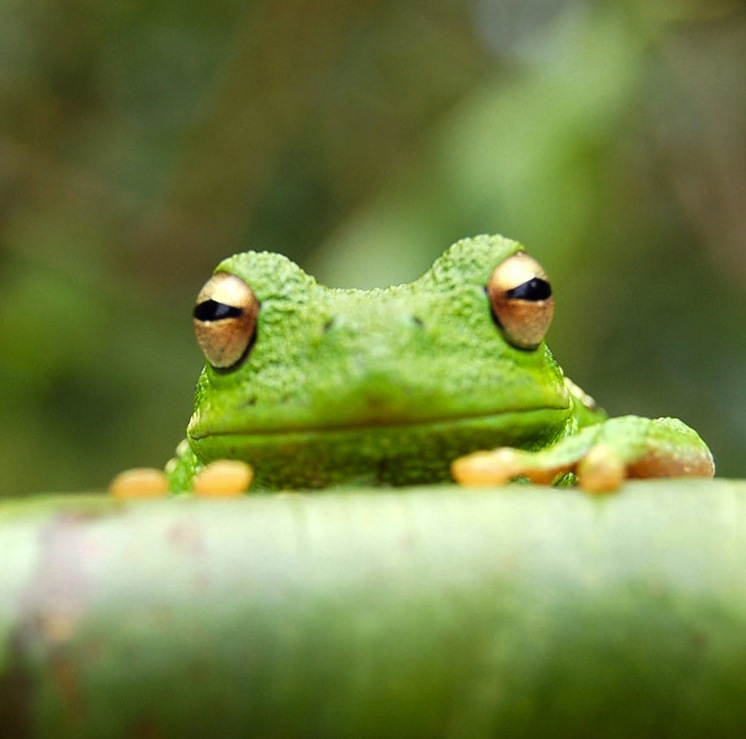
\includegraphics[width=0.3\textwidth]{frog.jpg}
%\caption{\label{fig:frog}This frog was uploaded via the project menu.}
%\end{figure}

\section*{Conclusions and Perspectives}
This project was focused on a specific stage, instead on the entire period of embryo brain development.
Thus, phylogenetics classification requires a deeper revision to determine the diversity of events in metazoa over the course of development. In fact, part of the aim of this project was an approach to explain how one brain developmental type could evolve into others.

Further analysis based on the relative timing and of the interdependence among major events and morphogenetic differences in early, mid and later  brain development in different metazoan groups must be performed.



\section*{References}
1-Gilbert S. F. (2006). Developmental Biology, 8th edn. Sunderland, MA: Sinauer Associates.\\
2-Carroll S. B., Grenier J. K., Weatherbee S. D. (2001). From DNA to Diversity: Molecular Genetics and the Evolution of Animal Design. Malden, MA: Blackwell Scientific.\\
3-Lynch V. J., Wagner G. P. (2008). Resurrecting the role of transcription factor change in developmental evolution. Evolution 62, 2131-2154.\\
4-Davidson E. H. (1991). Spatial mechanisms of gene regulation in metazoan embryos. Development 113, 1-26.\\
5-Davidson E. H., Peterson K. J., Cameron R. A. (1995). Origin of bilaterian body plans: evolution of developmental regulatory mechanisms. Science 270, 1319-1325. \\
6-Wray G. A. (2000). The evolution of embryonic patterning mechanisms in animals. Semin. Cell Dev. Biol. 11, 385-393.\\
7-Lechner M.,FindeiB S.,Steiner L., Marz M., Stadler P.F., Prohaska J.S. (2011).Proteinorto:Detection of(co) orthologs in large-scale analysis.BMC Bioinformatics 12,124.


\end{document}